\documentclass[tikz,border=8pt]{standalone}
\begin{document}
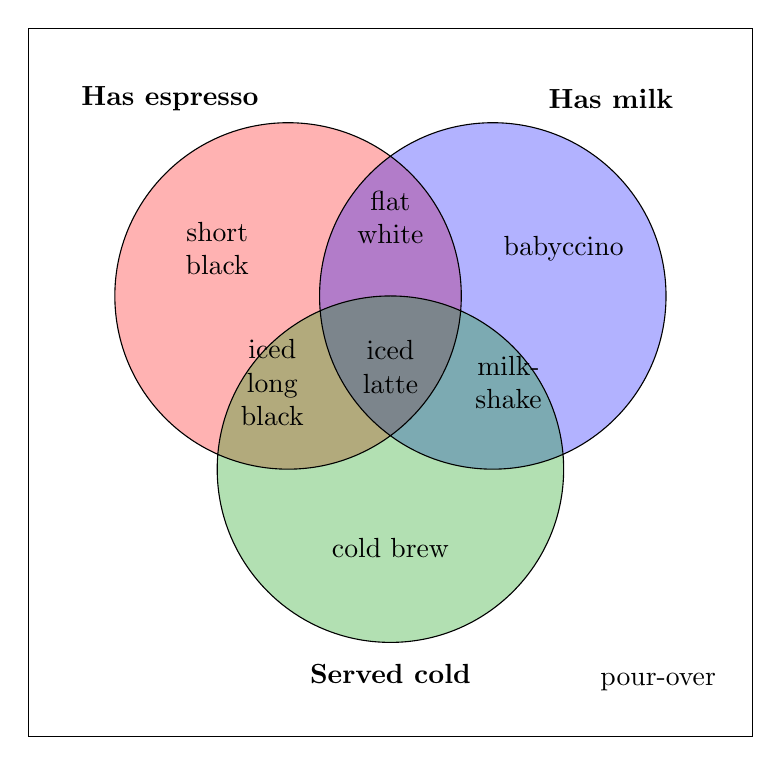
\begin{tikzpicture}
\draw (-4.6,-4.6) rectangle (4.6,4.4);
\begin{scope}[opacity=0.3]
\fill[red] (-1.3,1) circle (2.2);
\fill[blue] (1.3,1) circle (2.2);
\fill[green!60!black] (0,-1.2) circle (2.2);
\end{scope}
\draw (-1.3,1) circle (2.2) (1.3,1) circle (2.2) (0,-1.2) circle (2.2);
\node at (-2.8,3.5) {\bfseries Has espresso};
\node at (2.8,3.5) {\bfseries Has milk};
\node at (0,-3.8) {\bfseries Served cold};
\node[align=center] at (-2.2,1.6) {short\\black};
\node[align=center] at (2.2,1.6) {babyccino};
\node[align=center] at (0,-2.2) {cold brew};
\node[align=center] at (0,2.0) {flat\\white};
\node[align=center] at (-1.5,-0.1) {iced\\long\\black};
\node[align=center] at (1.5,-0.1) {milk-\\shake};
\node[align=center] at (0,0.1) {iced\\latte};
\node at (3.4,-3.9) {pour-over};
\end{tikzpicture}
\end{document}
